\chapter{Stakeholder Analysis} \label{ch:Stakeholder Analysis}

\begin{figure}[h]
    \centering
    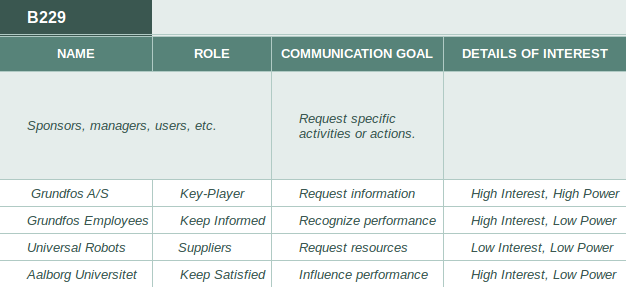
\includegraphics[scale=0.65]{StakeholderAnalysis/Stakeholder.png}
    \caption{Stakeholder Analysis} 
    \label{fig:Stakeholder} 
\end{figure}

\section{Grundfos A/S}\label{ch:grundfosas-stake}
Grundfos A/S is a stakeholder with high interest and high power, as they are investing in the UR. Their interest is high, because the further development of the robotic solution directly impacts the company. Development would be difficult without funding, which also gives Grundfos a lot of power. 


\section{Grundfos Employees}\label{ch:grundfosemp-stake}
Employees of Grundfos are stakeholders, who have a high interest, but a low influence.\\ The reason for this is, that they have no final say in whether the solution should be implemented. The Employees will in some instances have to learn new skills, in order to use the robots.


\section{Universal Robots}\label{ch:Universalrobots-stake}
The suppliers of the robotic manipulator in this case has a low interest and a low power, this is because they do not have any say in the matter. Whether it should be their manipulator or a competitors manipulator, they can then adjust the prices on the manipulator so we would choose their product for this case. 


\section{Aalborg University}\label{ch:Aau-stake}
Aalborg University has an interest in the development of robotics from a research and information perspective. For this reason they potentially have an interest in investing in further development and improvement of a technology such as the UR. 